After the global matrices assembly, the boundary conditions are applied. 
As was said in the section \ref{trimesh}, during the mesh import 
it is possible to identify the nodes that they are in the boundary. 
The condition where the nodes have their values predefined 
by the problem is known as \textit{Dirichlet condition}. 
Therefore, these nodes must not be changed as the simulation is 
performed. In this way, the product between the column of the 
global matrix whose index is a node with Dirichlet boundary condition 
and its predefined value as boundary condition is subtracted from 
the vector on the right side of the governing equation. 
Then, we zero the rows and columns of the global matrix that 
corresponds to the condition index of Dirichlet and we set the value 
of 1 on the main diagonal.

\medskip
For example, we will consider a matrix with (\textit{np x np}) size 
and node 2 as a node located on the domain boundary where 
the Dirichlet condition is proposed. 
Thus, the following algorithm is done as presented by Anjos (2007) 
\cite{anjos2007}:

\begin{enumerate}
 
 \vspace{0.5cm}
 \item \textbf{The boundary condition is located in the matrix:}
\medskip
\begin{center}
\begin{tikzpicture}
\matrix (m) [matrix of math nodes,
inner sep=0pt, column sep=0.4em,
nodes={inner sep=0.4em,text width=1.0em,align=center},
left delimiter={[},
right delimiter={]},
]
{
a_{11} & a_{12} & a_{13} & \cdots & a_{1j} & \cdots & a_{1n} \\
a_{21} & a_{22} & a_{23} & \cdots & a_{2j} & \cdots & a_{2n} \\
a_{31} & a_{32} & a_{33} & \cdots & a_{3j} & \cdots & a_{3n} \\
\vdots & \vdots & \vdots & \ddots & \vdots & \vdots & \vdots \\
a_{n1} & a_{n2} & a_{n3} & \cdots & a_{nj} & \cdots & a_{nn} \\
};
\begin{scope}[xshift=4.2cm]
\matrix (m) [matrix of math nodes,
inner sep=0pt, column sep=0.4em,
nodes={inner sep=0.4em,text width=1em,align=center},
left delimiter={[},
right delimiter={]},
]
{
c_1 \\
c_2 \\
c_3 \\
\vdots \\
c_n \\
};
\end{scope}
\begin{scope}[xshift=5.2cm]
\node {=};
\end{scope}
\begin{scope}[xshift=6.2cm]
\matrix (m) [matrix of math nodes,
inner sep=0pt, column sep=0.4em,
nodes={inner sep=0.3em,text width=0.8em,align=center},
left delimiter={[},
right delimiter={]},
]
{
b_1 \\
b_2 \\
b_3 \\
\vdots \\
b_n \\
};
\end{scope}
 \draw[<-] (-1.5,-1.8) -- (-1.5,-2.5) -- (-1.1,-2.5);
 \node [draw=none, align=right] at (2.0,-2.5) {Identify the column whose index is \\ Dirichlet condition};
\end{tikzpicture}
\end{center}

 \vspace{0.5cm}
 \item \textbf{Subtract the product between the column where the matrix node is 
located and its predefined value with the vector on the right hand side 
of the equation:}
\medskip
\begin{center}
\begin{tikzpicture}
\matrix (m) [matrix of math nodes,
inner sep=0pt, column sep=0.4em,
nodes={inner sep=0.4em,text width=1.0em,align=center},
left delimiter={[},
right delimiter={]},
]
{
a_{11} & a_{12} & a_{13} & \cdots & a_{1j} & \cdots & a_{1n} \\
a_{21} & a_{22} & a_{23} & \cdots & a_{2j} & \cdots & a_{2n} \\
a_{31} & a_{32} & a_{33} & \cdots & a_{3j} & \cdots & a_{3n} \\
\vdots & \vdots & \vdots & \ddots & \vdots & \vdots & \vdots \\
a_{n1} & a_{n2} & a_{n3} & \cdots & a_{nj} & \cdots & a_{nn} \\
};
\begin{scope}[xshift=4.2cm]
\matrix (m) [matrix of math nodes,
inner sep=0pt, column sep=0.4em,
nodes={inner sep=0.4em,text width=1em,align=center},
left delimiter={[},
right delimiter={]},
]
{
c_1 \\
c_2 \\
c_3 \\
\vdots \\
c_n \\
};
\end{scope}
\begin{scope}[xshift=5.2cm]
\node {=};
\end{scope}
\begin{scope}[xshift=6.2cm]
\matrix (m) [matrix of math nodes,
inner sep=0pt, column sep=0.4em,
nodes={inner sep=0.3em,text width=0.8em,align=center},
left delimiter={[},
right delimiter={]},
]
{
b_1 \\
b_2 \\
b_3 \\
\vdots \\
b_n \\
};
\end{scope}
 %text
 \draw[<-] (-1.5,-1.8) -- (-1.5,-2.5) -- (-1.1,-2.5);
 \node [draw=none, align=right] at (2.5,-2.5) {Subtract the product from this column with the \\ $c_2$ value on 
the right hand side of the equation};
 %block
 \draw[red] (-1.9,1.8) -- (-1.15,1.8) -- (-1.15,-1.7) -- (-1.9,-1.7) -- cycle;
 \draw[red] (3.9,0.95) -- (4.5,0.95) -- (4.5,0.45) -- (3.9,0.45) -- cycle;
\end{tikzpicture}
\end{center}

\newpage
that is,

\medskip
\begin{center}
\begin{tikzpicture}
\matrix (m) [matrix of math nodes,
inner sep=0pt, column sep=0.4em,
nodes={inner sep=0.4em,text width=1.0em,align=center},
left delimiter={[},
right delimiter={]},
]
{
a_{11} & a_{12} & a_{13} & \cdots & a_{1j} & \cdots & a_{1n} \\
a_{21} & a_{22} & a_{23} & \cdots & a_{2j} & \cdots & a_{2n} \\
a_{31} & a_{32} & a_{33} & \cdots & a_{3j} & \cdots & a_{3n} \\
\vdots & \vdots & \vdots & \ddots & \vdots & \vdots & \vdots \\
a_{n1} & a_{n2} & a_{n3} & \cdots & a_{nj} & \cdots & a_{nn} \\
};
\begin{scope}[xshift=4.2cm]
\matrix (m) [matrix of math nodes,
inner sep=0pt, column sep=0.4em,
nodes={inner sep=0.4em,text width=1em,align=center},
left delimiter={[},
right delimiter={]},
]
{
c_1 \\
c_2 \\
c_3 \\
\vdots \\
c_n \\
};
\end{scope}
\begin{scope}[xshift=5.2cm]
\node {=};
\end{scope}
\begin{scope}[xshift=6.2cm]
\matrix (m) [matrix of math nodes,
inner sep=0pt, column sep=0.4em,
nodes={inner sep=0.3em,text width=0.8em,align=center},
left delimiter={[},
right delimiter={]},
]
{
b_1 \\
b_2 \\
b_3 \\
\vdots \\
b_n \\
};
\end{scope}
\begin{scope}[xshift=7.2cm]
\node {-};
\end{scope}
\begin{scope}[xshift=8.2cm]
\matrix (m) [matrix of math nodes,
inner sep=0pt, column sep=0.4em,
nodes={inner sep=0.4em,text width=1em,align=center},
left delimiter={[},
right delimiter={]},
]
{
a_{12} \\
a_{22} \\
a_{32} \\
\vdots \\
a_{n2} \\
};
\end{scope}
\begin{scope}[xshift=9.0cm]
\node {*};
\end{scope}
\begin{scope}[xshift=9.4cm]
 \node {$c_2$};
\end{scope}
 %text
 \node [draw=none, align=right] at (8.5,-2.6) {$bc\_dirichlet$};
 %block
 \draw (7.3,-1.7) -- (7.3,-2.0) -- (9.7,-2.0) -- (9.7,-1.7);
 \draw (8.5,-2.0) -- (8.5,-2.3);
\end{tikzpicture}
\end{center}

 \vspace{0.5cm}
 \item \textbf{
The column and line of the boundary condition node index in matrix 
are filled with zeros:}
\medskip
\begin{center}
\begin{tikzpicture}
\matrix (m) [matrix of math nodes,
inner sep=0pt, column sep=0.4em,
nodes={inner sep=0.4em,text width=1.0em,align=center},
left delimiter={[},
right delimiter={]},
]
{
a_{11} & 0 & a_{13} & \cdots & a_{1j} & \cdots & a_{1n} \\
0 & 0 & 0 & \cdots & 0 & \cdots & 0 \\
a_{31} & 0 & a_{33} & \cdots & a_{3j} & \cdots & a_{3n} \\
\vdots & \vdots & \vdots & \ddots & \vdots & \vdots & \vdots \\
a_{n1} & 0 & a_{n3} & \cdots & a_{nj} & \cdots & a_{nn} \\
};
\begin{scope}[xshift=4.2cm]
\matrix (m) [matrix of math nodes,
inner sep=0pt, column sep=0.4em,
nodes={inner sep=0.4em,text width=1em,align=center},
left delimiter={[},
right delimiter={]},
]
{
c_1 \\
c_2 \\
c_3 \\
\vdots \\
c_n \\
};
\end{scope}
\begin{scope}[xshift=5.2cm]
\node {=};
\end{scope}
\begin{scope}[xshift=6.2cm]
\matrix (m) [matrix of math nodes,
inner sep=0pt, column sep=0.4em,
nodes={inner sep=0.3em,text width=0.8em,align=center},
left delimiter={[},
right delimiter={]},
]
{
b_1 \\
b_2 \\
b_3 \\
\vdots \\
b_n \\
};
\end{scope}
\begin{scope}[xshift=7.2cm]
\node {-};
\end{scope}
\begin{scope}[xshift=8.2cm]
\matrix (m) [matrix of math nodes,
inner sep=0pt, column sep=0.4em,
nodes={inner sep=0.4em,text width=1em,align=center},
left delimiter={[},
right delimiter={]},
]
{
a_{12} \\
a_{22} \\
a_{32} \\
\vdots \\
a_{n2} \\
};
\end{scope}
\begin{scope}[xshift=9.0cm]
\node {*};
\end{scope}
\begin{scope}[xshift=9.4cm]
 \node {$c_2$};
\end{scope}
\end{tikzpicture}
\end{center}


 \vspace{0.5cm}
 \item \textbf{One is placed on the main diagonal of the matrix whose
index is the boundary condition node:}
\medskip
\begin{center}
\begin{tikzpicture}
\matrix (m) [matrix of math nodes,
inner sep=0pt, column sep=0.4em,
nodes={inner sep=0.4em,text width=1.0em,align=center},
left delimiter={[},
right delimiter={]},
]
{
a_{11} & 0 & a_{13} & \cdots & a_{1j} & \cdots & a_{1n} \\
0 & 1 & 0 & \cdots & 0 & \cdots & 0 \\
a_{31} & 0 & a_{33} & \cdots & a_{3j} & \cdots & a_{3n} \\
\vdots & \vdots & \vdots & \ddots & \vdots & \vdots & \vdots \\
a_{n1} & 0 & a_{n3} & \cdots & a_{nj} & \cdots & a_{nn} \\
};
\begin{scope}[xshift=4.2cm]
\matrix (m) [matrix of math nodes,
inner sep=0pt, column sep=0.4em,
nodes={inner sep=0.4em,text width=1em,align=center},
left delimiter={[},
right delimiter={]},
]
{
c_1 \\
c_2 \\
c_3 \\
\vdots \\
c_n \\
};
\end{scope}
\begin{scope}[xshift=5.2cm]
\node {=};
\end{scope}
\begin{scope}[xshift=6.2cm]
\matrix (m) [matrix of math nodes,
inner sep=0pt, column sep=0.4em,
nodes={inner sep=0.3em,text width=0.8em,align=center},
left delimiter={[},
right delimiter={]},
]
{
b_1 \\
b_2 \\
b_3 \\
\vdots \\
b_n \\
};
\end{scope}
\begin{scope}[xshift=7.2cm]
\node {-};
\end{scope}
\begin{scope}[xshift=8.2cm]
\matrix (m) [matrix of math nodes,
inner sep=0pt, column sep=0.4em,
nodes={inner sep=0.4em,text width=1em,align=center},
left delimiter={[},
right delimiter={]},
]
{
a_{12} \\
a_{22} \\
a_{32} \\
\vdots \\
a_{n2} \\
};
\end{scope}
\begin{scope}[xshift=9.0cm]
\node {*};
\end{scope}
\begin{scope}[xshift=9.4cm]
 \node {$c_2$};
\end{scope}
\end{tikzpicture}
\end{center}

 \vspace{0.5cm}
 \item \textbf{The next nde is located and the step is performed again.}
\end{enumerate}

\newpage
\noindent
The implementation of this algorithm was performed by the following 
\textit{script}:

\begin{verbatim}
__________________________________________________________________________
 for mm in ibc:                        | boundary nodes loop
  bc_dirichlet -= LHS[:,mm]*bc_1[mm]   | step 2
  LHS[:,mm] = 0.0                      | step 3 - zero columns
  LHS[mm,:] = 0.0                      | step 3 - zero rows
  LHS[mm,mm] = 1.0                     | step 4 - one in main diagonal
  bc_dirichlet[mm] = bc_1[mm]          | computing the Dirichlet condition
__________________________________________________________________________
\end{verbatim}

\noindent
where \textit{ibc} is a list containing all the boundary nodes 
whose condition is Dirichlet and \textit{$bc\_1$} is an auxiliary 
vector with \textit{np} size where the value of the Dirichlet 
condition is computed in each index correspondence. 
The -= symbol ensures that the contribution of each node 
whose Dirichlet condition is computed. This procedure must be 
performed for each of the \textit{LHS}. The \ref{tempo contorno} 
shows the average processing time for the \textit{Dirichlet} 
condition apply in several unstructured linear triangular meshes.

\vspace{0.5cm}
\begin{table}[H]
\centering
\begin{tabular}{ccc}
\toprule
\textbf{Nodes} & \textbf{Elements} & \textbf{AVG Processing Time} (s) \\
\midrule
10482 & 20142 & 6,8 \\
40819 & 80005 & 37,5 \\
249677 & 495289 & 467,7 \\
993091 & 2010501 & 3720,6 \\
\bottomrule
\end{tabular}
\caption{Average processing time for Dirichlet condition in several unstrutured linear triangular meshes}
\label{tempo contorno}
\end{table}
 

\medskip
Another type of very common boundary condition is one
there is a flux in the domain boundaries. This boundary condition 
is known as \textit{Neumann condition} and in variational 
formulation it is called \textit{Natural condition}. 
Unlike the Dirichlet condition, this type of boundary condition 
does not affect the \textit{LHS} matrix when the flux is constant. 
We should only add their contribution to the vector on the right hand 
side of the equation, that is:

\begin{center}
\begin{tikzpicture}
\matrix (m) [matrix of math nodes,
inner sep=0pt, column sep=0.4em,
nodes={inner sep=0.4em,text width=1.0em,align=center},
left delimiter={[},
right delimiter={]},
]
{
a_{11} & 0 & a_{13} & \cdots & a_{1j} & \cdots & a_{1n} \\
0 & 1 & 0 & \cdots & 0 & \cdots & 0 \\
a_{31} & 0 & a_{33} & \cdots & a_{3j} & \cdots & a_{3n} \\
\vdots & \vdots & \vdots & \ddots & \vdots & \vdots & \vdots \\
a_{n1} & 0 & a_{n3} & \cdots & a_{nj} & \cdots & a_{nn} \\
};
\begin{scope}[xshift=4.2cm]
\matrix (m) [matrix of math nodes,
inner sep=0pt, column sep=0.4em,
nodes={inner sep=0.4em,text width=1em,align=center},
left delimiter={[},
right delimiter={]},
]
{
c_1 \\
c_2 \\
c_3 \\
\vdots \\
c_n \\
};
\end{scope}
\begin{scope}[xshift=5.2cm]
\node {=};
\end{scope}
\begin{scope}[xshift=6.2cm]
\matrix (m) [matrix of math nodes,
inner sep=0pt, column sep=0.4em,
nodes={inner sep=0.3em,text width=0.8em,align=center},
left delimiter={[},
right delimiter={]},
]
{
b_1 \\
b_2 \\
b_3 \\
\vdots \\
b_n \\
};
\end{scope}
\begin{scope}[xshift=7.2cm]
\node {-};
\end{scope}
\begin{scope}[xshift=8.2cm]
\matrix (m) [matrix of math nodes,
inner sep=0pt, column sep=0.4em,
nodes={inner sep=0.4em,text width=1em,align=center},
left delimiter={[},
right delimiter={]},
]
{
a_{12} \\
a_{22} \\
a_{32} \\
\vdots \\
a_{n2} \\
};
\end{scope}
\begin{scope}[xshift=9.0cm]
\node {*};
\end{scope}
\begin{scope}[xshift=9.4cm]
 \node {$c_2$};
\end{scope}
\begin{scope}[xshift=10.0cm]
\node {+};
\end{scope}
\begin{scope}[xshift=11.0cm]
\matrix (m) [matrix of math nodes,
inner sep=0pt, column sep=0.4em,
nodes={inner sep=0.4em,text width=1em,align=center},
left delimiter={[},
right delimiter={]},
]
{
ne_{1} \\
ne_{2} \\
ne_{3} \\
\vdots \\
ne_{n} \\
};
\end{scope}
 %text
 \node [draw=none, align=right] at (8.5,-2.6) {$bc\_dirichlet$};
 \node [draw=none, align=right] at (11.3,-2.6) {$bc\_neumann$};
 %block
 \draw (7.3,-1.7) -- (7.3,-2.0) -- (9.7,-2.0) -- (9.7,-1.7);
 \draw (8.5,-2.0) -- (8.5,-2.3);
 \draw (10.3,-1.7) -- (10.3,-2.0) -- (11.7,-2.0) -- (11.7,-1.7);
 \draw (11.0,-2.0) -- (11.0,-2.3);
\end{tikzpicture}
\end{center}

\medskip
As mentioned in the chapter \ref{metodo dos elementos finitos}, 
we have only Dirichlet condition in this work. Below, however, 
we will present the implementation of this type of condition. 
In order to exemplify, we will consider the boundary term 
of the equation \ref{diffusion2_concentration}, that is:

\begin{equation} 
 \frac{1}{\textit{ReSc}} \int_{\Gamma} \eta \nabla c \cdot \textbf{n} d\Gamma
\end{equation}

\medskip
\noindent
where $\nabla c$ is the flux that will be considered constant. 
After discretization by Galerkin formulation, we have the 
following expression:

\begin{equation} 
 \frac{1}{\textit{ReSc}} \int_{\Gamma} N_j \nabla c \cdot \textbf{n} d\Gamma
\end{equation}

\medskip
\noindent
that is:

\begin{equation} 
 \frac{1}{\textit{ReSc}} \Bigg[ \frac{length  \nabla c}{2} \Bigg]
\end{equation}

\medskip
\noindent
where the \textit{$length$} is the edge length of element. 
Whereas a two-dimensional domain, where 
\textit{$i$} is a boundary node, 
\textit{$i-1$} and \textit{$i+1$} are its neighbors nodes,
the edges of node
\textit{$i$} can be
shown as:

\begin{figure}[h!]
\begin{center}
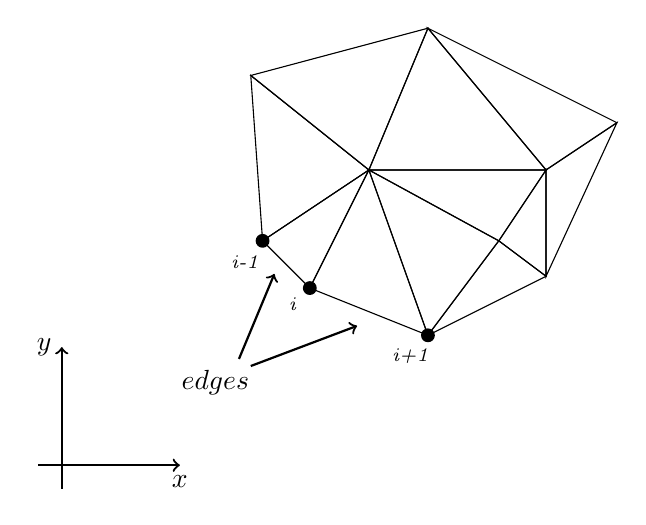
\begin{tikzpicture}[scale=3]
 \draw (0.75,0.75) -- (1.25,0.55) -- (1.00,1.25) -- cycle;
 \draw (0.75,0.75) -- (0.55,0.95) -- (1.00,1.25) -- cycle;
 \draw (1.25,0.55) -- (1.55,0.95) -- (1.00,1.25) -- cycle;
 \draw (1.55,0.95) -- (1.75,1.25) -- (1.00,1.25) -- cycle;
 \draw (1.75,1.25) -- (2.05,1.45) -- (1.25,1.85) -- cycle;
 \draw (1.25,1.85) -- (1.00,1.25) -- (1.75,1.25) -- cycle;
 \draw (1.25,0.55) -- (1.55,0.95) -- (1.75,0.80) -- cycle;
 \draw (1.55,0.95) -- (1.75,0.80) -- (1.75,1.25) -- cycle;
 \draw (1.75,0.80) -- (1.75,1.25) -- (2.05,1.45) -- cycle;
 \draw (0.55,0.95) -- (1.00,1.25) -- (0.50,1.65) -- cycle;
 \draw (1.00,1.25) -- (0.50,1.65) -- (1.25,1.85) -- cycle;
 \node[circle,fill=black, inner sep=0pt, minimum size=5pt] at (0.75,0.75) {};
 \node[circle,fill=black, inner sep=0pt, minimum size=5pt] at (0.55,0.95) {};
 \node[circle,fill=black, inner sep=0pt, minimum size=5pt] at (1.25,0.55) {};
 \node at (0.68,0.68) {\scriptsize \textit{i}};
 \node at (0.48,0.86) {\scriptsize \textit{i-1}};
 \node at (1.18,0.46) {\scriptsize \textit{i+1}};
 \draw [->,thick] (0.45,0.45)--(0.60,0.81);
 \draw [->,thick] (0.50,0.42)--(0.95,0.59);
 \draw [->,thick] (-0.3,-0.1)--(-0.3,0.5) node[left] {$y$};
 \draw [->,thick] (-0.4,0)--(0.2,0) node[below] {$x$};
 \node [draw=none] at (0.35,0.35) {$edges$};
\end{tikzpicture}
\end{center}
\caption{Edges of a node}
\end{figure}

\newpage
\noindent
where the left edge of the \textit{$i$} node is composed of 
\textit {$i-1$} and \textit {$i$}, while the right edge is composed 
of \textit {$i$} and \textit {$i+1$}. Thereby, we can observe 
that the node \textit {$i$} receives contribution from the its 
neighbors edges. The following \textit{script} is used to 
implement the Neumann boundary condition when required:

\begin{verbatim}
__________________________________________________________________________
 for i in range(0, len(neumann_edges)):   | boundary nodes loop
 
  p1 = neumann_edges[i][1]                | nodes of the edges
  p2 = neumann_edges[i][2]                | 

  x = x[p1] - x[p2]                       | 
  y = y[p1] - y[p2]                       | edge length calculation
  length = numpy.sqrt(x**2 + y**2)        | 

  bc_neumann[p1] += (length*nabla_c) / 2. | computing the Neumann
  bc_neumann[p2] += (length*nabla_c) / 2. | condition 
__________________________________________________________________________

\end{verbatim}

\noindent
where \textit{neumann\_edges} is a list containing the nodes 
presents on an edge whose condition is Neumann, \textit{p1} 
and \textit{p2} are the nodes presents on the edge, 
\textit{x} and \textit{y} are the coordinates of each node, 
\textit{length} is the edge length, \textit {nabla\_c} is the 
dimensionless flux modeled on the physical problem and 
\textit{numpy} is a numerical library of \textit{Python} 
in which we are using the square root function (\textit{numpy.sqrt}). 
The += symbol ensures that the contribution of the left and right 
edges is computed.
